%%%%%%%%%%%%%%%%%%%%%%%%%%%%%%%%%%%%%%%%%%%%%%%%%%%%%%%%%%%%%%%%%
%%% %
%%% % weiiszablon.tex
%%% % The Faculty of Electrical and Computer Engineering
%%% % Rzeszow University Of Technology diploma thesis Template
%%% % Szablon pracy dyplomowej Wydziału Elektrotechniki 
%%% % i Informatyki PRz
%%% % June, 2015
%%%%%%%%%%%%%%%%%%%%%%%%%%%%%%%%%%%%%%%%%%%%%%%%%%%%%%%%%%%%%%%%%

\documentclass[12pt,twoside]{article}
\usepackage[hidelinks]{hyperref}
\usepackage{weiiszablon}


\author{Motyka Beniamin}

% np. EF-123456, EN-654321, ...
\studentID{EF-160780}

\title{Bezpieczeństwo IT dla firm - opis i implementacja}
\titleEN{Temat pracy po angielsku}


%%% wybierz rodzaj pracy wpisując jeden z poniższych numerów: ...
% 1 = inżynierska	% BSc
% 2 = magisterska	% MSc
% 3 = doktorska		% PhD
%%% na miejsce zera w linijce poniżej
\newcommand{\rodzajPracyNo}{1}


%%% promotor
\supervisor{dr Michał Piętal}
%% przykład: dr hab. inż. Józef Nowak, prof. PRz

%%% promotor ze stopniami naukowymi po angielsku
\supervisorEN{(academic degree) Imię i nazwisko opiekuna}

\abstract{Treść streszczenia po polsku}
\abstractEN{Treść streszczenia po angielsku}

\begin{document}

% strona tytułowa
\maketitle

\blankpage

% spis treści
\tableofcontents

\clearpage
\blankpage

\clearpage
\section{Wprowadzenie}

W dzisiejszych czasach śmiało można stwierdzić, iż	Internet stał się ważną częścią ludzkiego istnienia. Niewątpliwy wpływ na ten stan rzeczy miała pandemia COVID-19 - sprawiła ona bowiem, że pewne dziedziny życia, takie jak dydaktyka czy praca wykonywana umysłowo, przeszły swoistą transformację. Miejsca, w których spotykali się studenci wraz z wykładowcami, czy pracownicy w biurze, stały się puste. Zastąpiła je komunikacja zdalna -- przez Internet.

Fakt, iż ludzkość została zmuszona, by przenieść znaczną część swojego funkcjonowania w sieć, niesie ze sobą poważne konsekwencje. Szybkie -- jak do tej pory -- tempo rozwijania się technologii informatycznych stało się nieporównywalnie bardziej dynamiczne, a co się z tym wiąże, obecne w sieci liczne zagrożenia stały się coraz powszechniejsze i trudniejsze w identyfikacji.

[coś tu jeszcze będzie]

\subsection{Cel i zakres pracy}

Celem niniejszej pracy inżynierskiej jest wyeksponowanie, opis oraz implementacja najbardziej pospolitych zagrożeń i luk bezpieczeństwa w Internecie nie tylko dla zwykłych użytkowników, ale również dla małych i średnich przedsiębiorstw. Dzięki temu, że powyższa idea zostanie zrealizowana w formie aplikacji e-learningowej, istnieje realna szansa na zwiększenie świadomości społecznej, edukację oraz poprawę zabezpieczeń systemów teleinformatycznych i infrastruktury sieciowej. Zakresem pracy są takie zagadnienia jak:
\begin{itemize}
\item Przegląd, dokumentacja i implementacja zagrożeń i luk bezpieczeństwa w sieci.
\item Stworzenie aplikacji e-learningowej przy użyciu technologii opisanych w kolejnym rozdziale. Użytkownicy będą mogli wziąć udział w interaktywnej prezentacji każdego z zagrożeń.
\item Zasugerowanie potencjalnych rozwiązań na opisane cyberzagrożenia.
\item Przedstawienie wniosków i implikacji płynących z powyższych.\\
\end{itemize} 
[coś tu jeszcze będzie]

\clearpage

\section{Technologie wykorzystane w aplikacji}
tekst 
\subsection{Javascript}
tekst 
\subsubsection{React.js}
tekst 
\subsubsection{Node.js}
tekst 
\subsection{GraphQL}
tekst 
\subsection{MongoDB}
tekst 

\clearpage
\section{Zagrożenia bezpieczeństwa}
tekst
\subsection{Phishing - opis}
tekst
\subsection{Phishing - przykład implementacji}
tekst 
\clearpage
\subsection{Ransomware - opis}
Ransomware to typ złośliwego oprogramowania, którego celem jest zablokowanie dostępu do komputera osobistego. Kiedy to złośliwe oprogramowanie dostanie się na urządzenie jako załącznik w wiadomości e-mail lub poprzez sieć, rozpoczyna proces szyfrowania asymetrycznego wszystkich plików. Czas trwania tej procedury zależy między innymi od wybranego algorytmu szyfrowania, jednak może wykonać się w czasie zaledwie pięciu godzin \cite{RansomwareTime}. Zazwyczaj ten czas jest znacznie dłuższy, gdyż przed rozpoczęciem procesu wymagany jest dokładny rekonesans systemu, w którym atakujący się znajduje. Tym sposobem użytkownik końcowy traci możliwość odczytu danych na swoim urządzeniu, a do odszyfrowania plików, wymagany jest klucz posiadany przez atakującego. 

Ten rodzaj szkodliwego oprogramowania jest szczególnie niebezpieczny dla przedsiębiorstw, gdyż utrata ważnych dokumentów czy danych finansowych, może się wiązać z poważnymi konsekwencjami. Celem ransomware nie jest usunięcie lub kradzież plików, ale zablokowane ich, i oczekiwanie na ewentualną spłatę okupu ze strony ofiary. 

Sposoby, poprzez które ransomware dostaje się do przedsiębiorstw, przedstawione są na poniższym rysunku, przygotowanym przez organizację CoveWare \cite{RansomwareAttackVectors}, która specjalizuje się w przeciwdziałaniu tego typu oprogramowaniu:
\begin{figure}[ht]
	\centering
	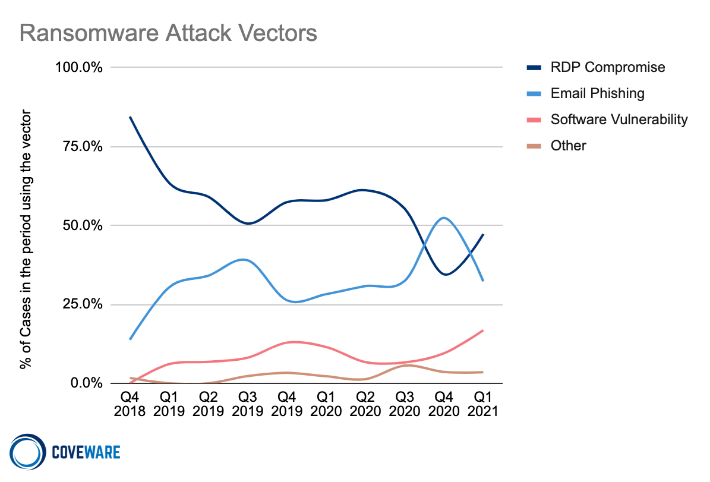
\includegraphics[width=13cm]{figures/ransomware-attack-vectors.png}
	\caption{Wektory ataku ransomware}
	\label{Fig:Wektory ataku ransomware}
\end{figure} 

Jak można zauważyć, wiodącym źródłem pozyskania tego złośliwego oprogramowania jest Remote Desktop Protocol (RDP) \cite{RDP} - protokół umożliwiający połączenie się z urządzeniem, oraz przejęcie nad nim pełnej kontroli, używany w firmach jako narzędzie do konfiguracji systemu dla pracowników. Zaraz za nim znajdują się maile phishingowe, opisane w poprzednim rozdziale, a następnie różnego rodzaju luki w oprogramowaniu. 

Najlepszą metodą przeciwko tego typu złośliwemu oprogramowaniu jest systematyczne wykonywanie archiwizacji danych. W tym wypadku, jeśli ransomware trafi do komputera i zaszyfruje wszystkie pliki, pozostaje jedynie odtworzyć kopię zapasową.

[coś tu jeszcze będzie]

\subsection{Ransomware - przykład implementacji}

tekst 

\subsection{Keylogger - opis}

Keyloggery występują zazwyczaj w formie złośliwego, ukrytego oprogramowania. Nie są widoczne na pierwszy rzut oka dla użytkownika i w zdecydowanej większości przypadków działają w tle, często podszywając się pod inną aplikację, tym samym maskując swoją obecność. 

Podstawowe właściwości tego typu złośliwego programu można opisać jako przejmowanie kontroli nad procedurami związanymi z obsługą klawiatury systemu operacyjnego, na którym się znajduje.

Głównym celem tego oprogramowania jest zbieranie danych o tym, jakie klawisze na klawiaturze zostały naciśnięte przez użytkownika, a następnie okresowe wysyłanie zebranych informacji do atakującego. Posiadając wiedzę na temat tego, co zostało wpisane na urządzeniu, można bez problemu uzyskać dostęp do wrażliwych informacji takich jak prywatna korespondencja czy poufne dane. Do bardziej zaawansowanych funkcji należy między innymi przesyłanie zrzutów ekranu, rejestrowanie historii otwieranych programów i przekazywanie tych informacji dalej.

Keyloggery oprócz formy programowej istnieją również jako osobne urządzenia, które podłączane są do jednostki zazwyczaj poprzez interfejs USB. Mogą także występować jako przejściówka pośrednicząca pomiędzy klawiaturą a złączem USB komputera. 

Sposobem na unikanie tego typu oprogramowania jest przede wszystkim systematyczne sprawdzanie uruchomionych procesów, ale także używanie odpowiedniego antywirusa.

\subsection{Keylogger - przykład implementacji}
tekst
\subsection{Wstrzyknięcie SQL - opis}
tekst
\subsection{Wstrzyknięcie SQL - przykład implementacji}
tekst
\subsection{DDOS - opis}
tekst
\subsection{DDOS - przykład implementacji}
tekst
\subsection{Ataki XSS - opis}

Cross-site scripting (XSS) jest jedną z najbardziej powszechnych podatności współczesnych aplikacji webowych.

Opisując XSS nie sposób nie wspomnieć o Regule tego samego pochodzenia (Same-origin policy) \cite{SameOriginPolicy}. Jest to jeden z wielu fundamentalnych mechanizmów bezpieczeństwa, zaimplementowany w każdej przeglądarce internetowej. Nie pozwala on żadnej stronie na podjęcie akcji lub odczytania zawartości innej strony, na przykład w dwóch kartach przeglądarki. W związku z tym, wszystko, co się dzieje na stronie internetowej otwartej przez użytkownika, jest izolowane, i nie będzie miało wpływu na pozostałe otwarte strony.

Cała struktura strony internetowej zakodowana językiem HTML może być zmieniana poprzez JavaScript, używając DOM API \cite{DOM}. Jako rezultat, prosty skrypt może całkowicie zmienić zawartość, wygląd, a przede wszystkim funkcjonalność strony internetowej.

Ciasteczkami \cite{Cookies} nazywa się niewielkie informacje wysyłane przez serwer do przeglądarki internetowej urządzenia końcowego. Służą temu, by zapisać obiekty danych w przeglądarce, które przy ponownym odwiedzeniu strony, mogą być przesłane do tego samego serwera, z którego przyszły. W związku z tym, przy odwiedzaniu różnorakich stron wymagających autoryzacji, użytkownik nie musi się za każdym razem logować, gdyż wszystkie potrzebne dane są zawarte w ciasteczkach, które przesyłane są razem z żądaniem.

XSS opiera się głównie na wstrzyknięciu do strony internetowej złośliwego skryptu, który, dla przykładu, może odczytać ciasteczka użytkownika lub inne poufne informacje, które przechowuje przeglądarka, wysłać je do atakującego, aby ten -- używając zapisanych w ciasteczkach danych -- mógł zalogować się na konto użytkownika, który nieświadomie uruchomił dany skrypt. Pomimo wielu zabezpieczeń, które są wbudowane w przeglądarki, te nie są w stanie odróżnić czy dany skrypt jest złośliwy, czy nie - dlatego też odporność aplikacji internetowej na tego typu atak stoi przede wszystkim po stronie programistów.

Najczęstszym miejscem, w którym można spotkać tę podatność, są formularze, do których użytkownik wpisuje jakąś treść, która następnie jest wyświetlana. Jeśli treść którą przesłał użytkownik nie zostanie odpowiednio okrojona, może dojść do sytuacji, w której to użytkownik wstrzyknie złośliwy skrypt.

[coś tu jeszcze będzie]

\subsection{Ataki XSS - przykład implementacji}
tekst
\subsection{Path Traversal - opis}

"Path Traversal" jest to nazwa dla powszechnej luki bezpieczeństwa aplikacji Internetowych, której niedopatrzenie, w procesie tworzenia oprogramowania, może skutkować w wycieku wrażliwych danych z serwera, na którym umieszczona jest aplikacja. 

Dzięki językom programowania działających po stronie serwera takim jak PHP zewnętrzne skrypty i pliki mogą być dołączane do aplikacji w sposób dynamiczny. Krytycznym elementem w tego typu funkcjonalnościach jest odpowiednio zaimplementowana logika dołączania plików oraz walidacja danych wejściowych, gdyż w przeciwnym wypadku, atakujący może odczytywać zawartość plików lokalnych, jak i zdalnych. Celem tej podatności jest zlokalizowanie i odpowiednie wykorzystanie parametrów przekazywanych do aplikacji, poprzez które dynamicznie dołączane są różne skrypty. 

Poniższy przykład prezentuje dołączenie pliku 'pl.php' jako parametr, celem ustawienia tekstu na stronie w języku polskim:

\url{http://samplepage.com/index.php?lang=pl.php}

Może to świadczyć o tym, że przyłączenie pliku do w kodzie źródłowym aplikacji wykonywane jest w następujący, przykładowy sposób:

\begin{lstlisting}[language=PHP,caption=Listing programu PHP,label={KodPHP1}]
	include($_GET['lang']);
\end{lstlisting}

Mając na uwadze fakt, że do aplikacji dynamicznie dołączany jest skrypt przekazywany w parametrze 'lang', atakujący może dokonać próby otworzenia zupełnie innego pliku, niż było to zakładane:

\url{http://samplepage.com/index.php?lang=../../../etc/passwd}

W rezultacie, zamiast wypisania tekstu w języku polskim, przekazana zostanie zawartość pliku `/etc/passwd`, w którym to znajdują się informacje o wszystkich użytkownikach w systemie.

[coś tu jeszcze będzie]

Aby zapobiec tej luce, zamiast wykluczać lub usuwać dane ciągi znaków należy odpowiednio sprawdzać dane wejściowe i zezwalać jedynie na wybrane znaki, lub ciągi znaków, na przykład z wykorzystaniem wyrażeń regularnych. 

\subsection{Path Traversal - przykład implementacji}
tekst
\subsection{Spoofing - opis}
tekst
\subsection{Spoofing - przykład implementacji}
tekst
\clearpage
\section{Podsumowanie i wnioski końcowe}



\clearpage

\addcontentsline{toc}{section}{Literatura}

\begin{thebibliography}{4}
\bibitem{sekurak} Securitum. Bezpieczeństwo aplikacji webowych
\bibitem{SameOriginPolicy} https://developer.mozilla.org/en-US/docs/Web/Security/Same-origin{\_}policy
\bibitem{DOM} https://developer.mozilla.org/en-US/docs/Web/API/Document{\_}Object{\_}Model. 
\bibitem{Cookies} https://developer.mozilla.org/en-US/docs/Web/HTTP/Cookies. 
\bibitem{RDP} https://docs.microsoft.com/en-us/troubleshoot/windows-server/remote/understanding-remote-desktop-protocol
\bibitem{RansomwareAttackVectors} https://www.coveware.com/blog/ransomware-attack-vectors-shift-as-new-software-vulnerability-exploits-abound
\bibitem{RansomwareTime} https://thedfirreport.com/2020/10/18/ryuk-in-5-hours/
\bibitem{Ddos} https://www.cloudflare.com/learning/ddos/what-is-a-ddos-attack/

\end{thebibliography}

\clearpage

\makesummary

\end{document} 
